%%%%%%%%%%%%%%%%%%%%%%%%%%%%%%%%%%%%%%%%%%%%%%%%%%%%%%%%%%%%%%%%%%%%%%%%%
%
% Time
%
%%%%%%%%%%%%%%%%%%%%%%%%%%%%%%%%%%%%%%%%%%%%%%%%%%%%%%%%%%%%%%%%%%%%%%%%%




%Time in databases: temporal databases: the crisp stuff. General things.
\subsection{\label{subsec:time-in-databases}Time in Databases}
The concept of adding time to databases has been profoundly studied~\cite{Darwen1998},~\cite{Etzion1998},~\cite{Etzion1998b},~\cite{Gal1998},~\cite{Jensen1999},~\cite{Lomet2006},~\cite{Nascimento1995},~\cite{Sarda1990},~\cite{Snodgrass1998},~\cite{Toman1998},~\cite{Wu1998}. A true standard for adding temporal aspects to relational databases does not exist, but there is a consensus on what is called a \emph{temporal database}: a temporal database is a database that supports some aspects of time~\cite{Dyreson1994}. Thus, a temporal database will contain data representing \emph{temporal values}. Notions of time, such as instants~\cite{Dyreson1994}, time intervals~\cite{Dyreson1994} or temporal elements~\cite{Dyreson1994} are generally called `temporal values' in the context of temporal databases. Based on their interpretation and modelling purpose, time notions and the corresponding times can be classified into four types. Of these types, \emph{user-defined time} comprises time indications of which the modelling has no impact on the consistency of the temporal database. The data representing these temporal values are not handled differently from data of non-temporal attributes (by the temporal DBMS)~\cite{Dyreson1994}. The other types contain time indications typically represented by data which are handled exceptionally by the temporal DBMS. The definitions and explanations of these types can be found in~\cite{Dyreson1994} and~\cite{Nascimento1995} and more information can be found in~\cite{Jensen1991},~\cite{Snodgrass1984} and~\cite{Nascimento1995}.

\begin{itemize}
	\item \emph{Valid time}: The \emph{valid-time} (VT) of a fact is the time when the fact is true in the modeled reality~\cite{Dyreson1994}.
	\item \emph{Transaction time}: A database fact is stored in a database at some point in time, and after it is stored, it is current until logically deleted. The \emph{transaction-time} (TT) of a database fact is the time when the fact is current in the database and may be retrieved~\cite{Dyreson1994}.
	\item \emph{Decision time}: The \emph{Decision time} (DT) of an event is the time when an event was decided to happen~\cite{Nascimento1995}.
\end{itemize}

An example: consider a database containing data representing the capacities of various aspects of employee contracts. The time during which an employee's contract is valid and the employee is hired, will then be VT. The moment on which an employee's contract is stored in the database, will then be TT. The time when the decision for hiring this employee was made, will then be DT.

Depending on the time represented in the database, a database is classified as either a \emph{valid-time database} (VTDB), a \emph{transaction-time database} (TTDB), a \emph{decision-time database} (DTDB), a \emph{bitemporal database} (both valid-time indications and transaction-time indications are represented), or a \emph{tritemporal} or \emph{multitemporal database} (valid-time indications, transaction-time indications and decision-time indications are represented).

%Now in the context of a relational database: what is a VT/TT/... relation? We will use VT relations, thus we should explain what they are.
In the context of relational databases, more specific definitions exist. For example, a \emph{valid-time relational database} is a relational database containing one or more \emph{valid-time relations}, a \emph{transaction-time relational database} is a relational database containing one or more \emph{transaction-time relations} and a \emph{bitemporal relational database} is a relational database containing one or more \emph{bitemporal relations}~\cite{Dyreson1994}. A valid-time relation is then a relation with exactly one system-supported VT, a transaction-time relation is a relation with exactly one system-supported TT and a bitemporal relation is a relation with exactly one system-supported VT and exactly one system-supported TT~\cite{Dyreson1994}. The attributes used in a valid-time relation to describe VT are called \emph{valid-time attributes}. The attributes used in a transaction-time relation to describe TT are called \emph{transaction-time attributes}. Any attribute unrelated to VT, TT or DT is usually called a \emph{non-temporal attribute}.


%In a temporal database system, a \emph{chronon} is the shortest duration of time supported by the system. % is a non-decomposable unit of time.  it  There are two ways to represent a chronon: as a point or as an interval \cite{655777}. %WE NEVER USE CHRONONS IN THIS PAPER!
Typically, when time modelling is supported by a database system, some behavioral aspects of the database model are extended or enhanced and some extra behavioral aspects are introduced, to deal with possible temporal inconsistencies and to allow more complex (temporal) queries. The presented work only deals with valid-time relational databases. In the presented work, a general extended/enhanced version of the relational database model is used. This extended version is based on several works, mainly the work presented in~\cite{Jensen1994}. In subsection~\ref{subsubsec:Understanding-valid-time-databases}, the extensions to the relational database model used in this work are presented on a logical level, but first, in subsection~\ref{example-situation}, an example situation is presented, which will be used throughout this paper to explain the various concepts treated in light of the presented work.


%Thus, in the presented work, an extended version of the Data Manipulation Language DML, which is part of the standard database querying language SQL, is used. This extended version is based on several works, mainly the work presented in~\cite{Jensen1994}. In subsection~\ref{subsubsec:Understanding-valid-time-databases}, the extensions to the DML used in this work are presented, but first, in subsection~\ref{example-situation}, an example situation is presented, which will be used throughout this paper to explain the various concepts treated in light of the presented work.

\subsection{\label{example-situation}Example Situation}
Consider a valid-time relation modelling the absence through loaning of books in a library. The relation contains 4 attributes: `ID', `Title', `Start Loan' and `End Loan'. Every physical book is given a unique identifier. This identifier is represented by a number and described by attribute `ID'. Attribute `Title' describes the title of a book. Attributes `Start Loan' and `End Loan' describe the starting date, respectively ending date on which a valid-time interval starts, respectively ends. This time interval is the time interval during which the book, represented by the value of the tuple for the `ID' attribute, was loaned to a customer. Table \ref{tbl:library-sample} visualises this relation with a few tuples in the relation extention.

\tcap{\label{tbl:library-sample}Example library relation.}
%\centerline{\small DATA TYPES}
\vglue-6pt
\centerline{\small\baselineskip=13pt
\begin{tabular}{c c c c}\\
\hline
\textbf{ID}  & Title  & Start Loan & End Loan \\
\hline
3 & Dracula & 15/3/2012 & 30/3/2012 \\
4 & Frankenstein & 25/3/2012 & 4/4/2012 \\
5 & Harry Potter & 18/3/2012 & 2/4/2012\\
3 & Dracula & 4/4/2012 & UC \\
\hline\\
\end{tabular}
}

%Valid-time databases and relations: general things AND an explanation about the exact things we will use in the rest of the paper. (+ vocabulary/concept explanation). Also explain the working of crisp valid-time databases/relations.
\subsection{\label{subsubsec:Understanding-valid-time-databases}General Valid-time Databases}
This subsection is devoted to describing the general behavior of general valid-time relational databases. This behavior will be described on a logical level, by (logically) defining and describing general forms of the four basic functions typically present in any relational database model. These functions are `create', `read', `update' and `delete' and will be denoted `the CRUD functions'. Usually, the CRUD functions in a valid-time relational database model are defined using the CRUD functions in a non-temporal relational database model. For example, the update function in a valid-time relational database model will typically be defined using several non-temporal create and update functions. In the presented work, the CRUD functions in the non-temporal relational database model will be given a subscript `NT', while the CRUD functions in the valid-time relational database model will be given a subscript `VT'.

Before defining and describing the CRUD functions used in the presented work, some concepts should be described and defined and the corresponding terminology and denotation style of these concepts should be determined. 

%For the sake of simplicity, only the three main operations in the Data Manipulation Language \emph{DML} a.k.a \emph{CRUD} (CReate Update, Delete) operations are shown. Usually the DML operations in a temporal database are re-defined e.g. a typical update sentence in SQL could be re-defined by means of several insert and update sentences. Therefore, in order to be clear, these high level primitives in the DML for a valid-time database are usually noted as Insert, Modify and Delete. In the following subsections each primitive is defined and explained. Finally a illustrative example is given. For a more complete information on the behaviour of a bitemporal database, please refer to ~\cite{Jensen1994}.

Every valid-time relation has one VT. In the presented work, indications of VT which are represented in a valid-time relation are always time intervals. In the presented work, such a valid-time interval is represented in the valid-time relation using two instants~\cite{Dyreson1994}: a starting instant and an ending instant.

Consider a valid-time relation $R$ with attribute tuple $\left(A_{0},\ A_{1},\ A_{2},\ \ldots,\ A_{n},\ Start,\ End\right)$, where every $A_{i}$, $i \in \Nat$ and $i \geq 1$ and $i \leq n$ and $n \in \Nat_{0}$, denotes a non-temporal attribute and where $Start$ and $End$ denote temporal attributes, respectively describing starting and ending instants. Now consider an entity $E$ of which the properties are described by the aforementioned attributes $A_{i}$ and a time interval $I$ defined by instants $I_{s} \text{ and } I_{e}$ where $I_{s}$ and $I_{e}$ denote instants. Let the values representing these instants be denoted $s \in \T$ and $e \in \T$ respectively, $\T$ being the domain of the temporal attributes and let the representation of the time interval I be denoted $\left[s,\ e\right]$. Let the value representing the state of $E$ for attribute $A_{i}$ during time interval $I$ be denoted $a_{i}$, for every $i \in \Nat$ for which $i \geq 1$, $i \leq n$, and let the n+1-tuple $\left(a_{0},\ a_{1},\ a_{2},\ \ldots,\ a_{n}\right)$ be denoted $a$. The denotation 

\begin{equation}
\label{eq:def-state}
\left(a,\ \left[s,\ e\right]\right)
\end{equation}

now expresses that the state of $E$ represented by $a$ is valid in the modelled reality during time interval $I$. This denotation is also used to indicate the n+3-tuple $\left(a_{0},\ a_{1},\ a_{2},\ \ldots,\ a_{n},\ s,\ e\right)$. The denotation

\begin{equation}
\label{eq:def-element}
\left(R,\ \left(a,\ \left[s,\ e\right]\right)\right)
\end{equation}

now expresses that the n+3-tuple $\left(a,\ \left[s,\ e\right]\right)$ = $\left(a_{0},\ a_{1},\ a_{2},\ \ldots,\ a_{n},\ s,\ e\right)$ is an element of the extention of $R$.

%\begin{definition}
%Consider a relation $R$ in a temporal database, an entity $A$ given by the attributes $\left(a_1, \ldots, a_n \right)$ and the crisp time interval $I$ given by $\left[a,\ b\right] : a,b \in \T, a \leq b$. The pair $\left(A, I\right)$ expresses that the data regarding the entity A is valid during the crisp time interval I.  Note that the relation $R = \left(A, I \right) x \left(A, I \right)$. The following equation indicates that the pair $\left(A, I\right)$ is in the relation R:
%\begin{equation}
%\label{eq:rel-def}
%\left( R, \left(A , I\right) \right)
%\end{equation}
%\end{definition}

%\begin{example} \textcolor{red}{TODO: INTEGRATE THIS EXAMPLE IN THE `GENERAL EXAMPLE'}
%\label{ex:library-database}
%Consider a library database. Each physical book is stored with an identifier (ID), a title and the start and end loan dates respectively. Table \ref{tbl:library-sample} illustrates the first version of the database, after three insertions. In this example, $A = ($ ID, Title $)$ and $I = ($ Start Loan, End Loan $)$.
%\end{example}

%\vglue13pt
%\begin{table}[htbp]



%In order to simplify the algorithms for the manipulation of data, some auxiliary functions and constants are defined:
In order to simplify the definition of the CRUD functions, some auxiliary functions and constants are first defined.

For the valid-time relation $R$ to be able to represent that the state of entity $E$, represented by $a$, is currently valid, the time domain used by the temporal attributes ($Start$ and $End$) should contain a special constant called \emph{Until Changed} (\emph{UC}).

\begin{definition}
 \label{def:until-changed}
\textbf{Until Changed (\emph{UC}).}\\
Given a time domain $\T$, \emph{Until Changed} is a single value in $\T$ representing an instant infinitely far in the future.
\end{definition}
\vspace{10pt}

This constant is special in that sense that if the value of a tuple of $R$ for attribute $End$ is $UC$, the state, represented by the values of this tuple for the non-temporal attributes, is considered to be valid currently and during an unlimited amount of time in the future.


%To show that the data related to the entity $\left(A, I \right)$ is up-to-date, a special constant called \emph{Until Changed} is defined for the endpoint, $d$, of the time interval $I = \left(c, d\right)$. The value for this constant is considered to be $+\infty$. 

\begin{definition}
\label{def:current-tuple}
\textbf{Current Tuple.}\\
The n+1-tuple $a$ is \emph{current} in relation $R$ if and only if:

\begin{equation}
\exists\ c\ \in\ \T|\ \left(R,\ \left(a,\ \left[c,\ UC\right]\right)\right) \nonumber
\end{equation} 

\end{definition}

%If the pair $\left(A, I \right)$ with $I = \left(c, UC \right), c \in \T$ is in the relation $R$, then, it is said that the pair $\left(A, I \right)$ is \emph{current} in the relation.

For example, the last row in Table \ref{tbl:library-sample} visualizes the values representing a time interval $\left[4/4/2012 , UC \right]$. The interpretation is that the book with ID = 3 was loaned on 4/4/2012 and it is still loaned. The tuple representing the book with ID = 3 is current in the relation.

The concepts above now allow the introduction of the function \emph{Current}:

\begin{align}
\text{Current} & :\ \Rel \times R_{NT} & \rightarrow & Ex_{R} \nonumber \\
               & :\ \left(R,\ a\right) & \rightarrow &
 \begin{cases}
  \left\{\left(a,\ \left[s,\ e\right]\right)\right\} & \text{if } \exists \left(a,\ \left[s,\ e\right]\right)| \\
  									 & (\left(R,\ \left(a,\ \left[s,\ e\right]\right)\right)\\
  									 & \wedge \left(\left[s,\ e\right]\ =\ \left[c,\ UC\right]\right)), \\
  									 & c \in \T \\
  \emptyset & \text{else}
 \end{cases}
 \nonumber
\end{align}

Here, $Ex_{R}$ denotes the extention of $R$, $\Rel$ denotes the set of all relations in the database schema and $A_{NT}$ denotes the set of all n+1-tuples consisting of the non-temporal values of the tuples of relation $R$.

%\begin{definition}
%\label{def:current-in-relation}
%\textbf{Function `Current'.}\\

%This function returns a crisp time interval $I$ if the entity $A$ is current in the relation $R$ or the empty set, if the entity $A$ is not current in the relation.

%Consider an object $A$ and a relation $R$ in a temporal database. The function Current$\left(R, A \right)$ obtains the tuple $\left(A, I \right)$ that is current in the relation $R$, that is it, $I = \left[a, +\infty \right]$.

%\begin{align}
%\label{eq:current-in-relation}
%\mbox{Current} \left(R, A \right) &=& \\ 
%\begin{cases}
%\nonumber
%I & \mbox{ if } (A,I) \in R \wedge I = \left(c, UC \right), c \in \T\\
%\emptyset & \mbox{ in any other case }
%\end{cases}
%\end{align}
%\end{definition}

For example, the expression Current($R_{ex}$, $\left\{3,`Dracula'\right\}$), where $R_{ex}$ denotes the example relation visualized in table \ref{tbl:library-sample}, returns the tuple $\left\{3, `Dracula', 4/4/2012 , UC\right\}$. On the other hand, Current($R_{ex}$, $\left\{4,`Frankenstein'\right\}$) returns the empty set.

%The following two Allen's relations (see Figure \ref{fig:allen-rel}) are defined~\cite{Nagypal2003} to implement the auxiliary functions. 

Given two time intervals $I$, represented by $\left[s_{I},\ e_{I}\right]$, and $J$, represented by $\left[s_{J},\ e_{J}\right]$, the following two functions \emph{During} and \emph{Overlaps} are functions used to compare the time intervals $I$ and $J$, based on sequential comparisons of the values representing their starting and ending instants.


\begin{align}
\text{During} & :\ \Pow(\T)\ \times\ \Pow(\T) & \rightarrow & \bool \nonumber \\
              & :\ \left(\left[s_{I},\ e_{I}\right],\ \left[s_{J},\ e_{J}\right]\right) & \rightarrow & \left(s_{I}\ >\ s_{J}\right)\ \wedge\ \left(e_{I}\ <\ e_{J}\right)
              \nonumber
\end{align}

\begin{align}
\text{Overlaps} & :\ \Pow(\T)\ \times\ \Pow(\T) & \rightarrow & \bool \nonumber \\
							  & :\ \left(\left[s_{I},\ e_{I}\right],\ \left[s_{J},\ e_{J}\right]\right) & \rightarrow & \left(s_{I}\ <\ s_{J}\right)\ \wedge\ \left(e_{I}\ <\ e_{J}\right)\nonumber \\
							  & & & \wedge\ \left(e_{I}\ >\ s_{J}\right)
							  \nonumber
\end{align}

Here, $\Pow(\T)$ is the powerset of $\T$ and $\bool$ is the Boolean domain $\bool\ =\ \left\{T,\ F\right\}$, where $T$ is a value representing the logical constant `True' and $F$ is a value representing the logical constant `False'. Now, the function \emph{CloseR} can be introduced. CloseR is used to `close' the representation of a time interval with respect to the representation of another time interval.

\begin{align}
\text{CloseR} & :\ \Pow(\T)\ \times\ \Pow(\T) & \rightarrow & \Pow(\T) \nonumber \\
							& :\ \left(\left[s_{I},\ e_{I}\right],\ \left[s_{J},\ e_{J}\right]\right) & \rightarrow & 
							\begin{cases}
							\left[s_{I},\ s_{J}\right[ & \text{if } \left(s_{J}\ =\ UC\right)\ \wedge\\
							 & \text{During}(\left[s_{J},\ e_{J}\right], \\
							 & \left[s_{I},\ e_{I}\right]) \\
							\left[s_{I},\ e_{I}\right] & \text{else }
							\end{cases}
							\nonumber
\end{align}

For example, consider two time intervals, represented by $I = \left[4/4/2012, UC \right]$ and $J = \left[24/4/2012, UC \right]$ respectively. Then, CloseR$\left(I, J \right) = \left[4/4/2012, 23/4/2012 \right]$.




%Analogously, it is defined the function to close a left-open interval: 
%\begin{definition}
%\label{def:close-a-crisp-interval-l}
%CloseL$\left(I, J\right)$ 
%\begin{align}
%\mbox{CloseL} \left( I, J \right) &=& \\ 
%\begin{cases}
%\nonumber
%I & \mbox{ if } a \neq -\infty \\
%I=\left]d, b \right] & \mbox{ if } a = -\infty \wedge J < I
%\end{cases}
%\end{align}
%\end{definition}




%\begin{definition}
%\label{def:first-in-relation}
%Analogously, the function First$\left(R, A \right)$ obtains the tuple $\left(A, I \right)$ where $I$ is a right-open interval and which is the first version in the relation $R$, that is it, $I = \left[-\infty, b \right]$.
%\begin{align}
%\label{eq:first-in-relation}
%\mbox{First} \left(R, A \right) &=& \\ 
%\begin{cases}
%\nonumber
%I & \mbox{ if } \exists b \in I : (A,I) \in R \wedge a = -\infty \\
%\emptyset & \mbox{ in any other case }
%\end{cases}
%\end{align}
%
%\end{definition}



The functionality provided by functions Current and CloseR now allows to introduce the necessary CRUD-functions.


%Now it is possible to `close' the current version of an entity by using \eqref{eq:close-a-crisp-interval} and \eqref{eq:current-in-relation}. This functionality is required to append new information about an existing entity in the relation.

%\begin{definition}
%\label{def:close-current-version}
%Consider an entity $A$, the relation $R$ and a time interval $J$. Then, the function close-current$\left(R,\left(A,J\right) \right)$ closes any current version of the object $A$ if it exists and add the new version $\left(A, J \right)$.

%\begin{eqnarray}
%\label{eq:close-current}
%\text{Close-current} \left(R, \left(A, J\right) \right) =\\
%\begin{cases}
%\nonumber
%R - \left(A, I \right) \cup \left \lbrace \left(A, \mbox{ CloseR } \left(I, J\right) \right)\right \rbrace \cup \left \lbrace\left(A, J\right) \right \rbrace  \\
%\nonumber
%\mbox{ if } I = \mbox{ Current } \left(R, A \right)\\ %\wedge J > \mbox{ CloseR } \left(I, J \right)   \\
%\nonumber R , \text{ in any other case}
%\end{cases}
%\end{eqnarray}
%\end{definition}

%For example, consider the book with ID = 3 in Table \ref{tbl:library-sample}. The current version was loaned on 4/4/2012. The book was returned to the library but, for some reason, the end loan date was not registered. The book is loaned again on 24/4/2012. Then, the Close-current function allows to close the current version of the book and insert a new version. First, the function CloseR is applied with $I = \left(4/4/2012, UC \right)$ and $J = \left(24/4/2012, UC \right)$. Hence, the value for the time interval $I$ is $ \left(4/4/2012, 23/4/2012 \right)$. Then, the modifications on the value for the time interval $I$ are stored. Finally, a new row with the current values of the book and the time interval $J$ is stored.
%The result of this operation is illustrated on Table \ref{tbl:library-sample-2}.




%It is also possible to append at the beggining by using \eqref{def:close-a-crisp-interval-l} and \eqref{def:first-in-relation}.
%\begin{definition}
%\label{def:append-first-version}
%Consider an object $A$, the relation $R$ and a time interval $J$. Then, the function append-first$\left(R,A,J \right)$ closes any right open version of the object $A$ if it exists and add the new version $\left(A, J \right)$.
%
%\begin{eqnarray}
%%\label{eq:close-current}
%\text{Append-first} \left(R, A, J \right) =\\
%\begin{cases}
%\nonumber
%\big \lbrace R - \left(A, I \right) \cup \left \lbrace \left(A, \mbox{ CloseL } \left(I, J\right) \right) \cup \left(A, J\right)\right \rbrace  \big \rbrace \\
%\nonumber
%\mbox{ if } I = \mbox{ First } \left(R, A \right) \wedge J < \mbox{ CloseL } \left(I, J \right)   \\
%\nonumber R , \text{ in any other case}
%\end{cases}
%\end{eqnarray}
%\end{definition}
\subsubsection{\label{subsubsec:modify}CRUD function `update'}
This operation adds new information about an existing entity $E$ in the relation $R$. The update function does not remove any previous information about $E$, but it `closes' the current version for the entity $E$ and adds a new version.


%Note that the modify operation is only applicable when the object $A$ is current in the relation $R$; $ \left(A, I \right) \in R, I = \left[a, +\infty \right]$.

\begin{align}
\text{update}_{VT} & :\ \Rel\ \times\ Ex_{R} & \rightarrow & \Rel \nonumber \\
							& :\ \left(R,\ \left(a,\ \left[s_{J},\ e_{J}\right]\right)\right) & \rightarrow & 
							\begin{cases}
							COND & \text{if } \\
							& Current(R,\ a)\ \neq\ \emptyset \\							
							R & \text{else }
							\end{cases}
							\nonumber
\end{align}

Here, COND stands for the expression:

\begin{align}
& \left(Ex_{R}\ \backslash\ Current\left(R,\ a\right)\right) \nonumber \\
& \cup\ \left\{\left(a,\ CloseR\left(\left[c,\ UC\right],\ \left[s_{J},\ e_{J}\right]\right)\right)\right\} \nonumber \\
& \cup\ \left\{\left(a,\ \left[s_{J},\ e_{J}\right]\right)\right\} \nonumber
\end{align}

In all of this, the `previous' version of the entity was valid during the time interval represented by $\left[c,\ UC\right]$ and the `new' version of the entity is valid during the time interval represented by $\left[s_{J},\ e_{J}\right]$.

%\begin{align}
%\label{eq:modify}
%\MOD \left( R, \left(A, I \right)\right) =\\
%\begin{cases}
%\nonumber
%\mbox{ Close-current }\left(R, \left(A, I\right) \right) %\\
% \mbox{ if Current}\left(R ,A \right) \neq \emptyset \\
% R,  \mbox{ otherwise }
%\end{cases}
%\end{align}


\subsubsection{\label{subsubsec:insert}CRUD function `create'}
The purpose of this function is to allow storing data describing an entity $E$ which is valid during the time interval represented by $\left[s_{I},\ e_{I}\right]$. The exact behavior of this function depends on the situation of the relation $R$. Two main possibilities exist.
\begin{enumerate}
\item The entity $E$ was never represented by any tuple in $R$. In this case, a tuple is simply added to the extention of $R$, representing the state of $E$ during $\left[s_{I},\ e_{I}\right]$. %: The object is added with the valid-time indicated by the crisp interval $I$. In the example, this correspond with the following insertion sentences:

\begin{align}
\text{create}_{VT} & :\ \Rel\ \times\ Ex_{R} & \rightarrow & \Rel \nonumber \\
							& :\ \left(R,\ \left(a,\ \left[s_{I},\ e_{I}\right]\right)\right) & \rightarrow \nonumber \\ 
							& create_{NT}\left(R,\ \left(a,\ \left[s_{I},\ e_{I}\right]\right)\right)
							\nonumber
\end{align}

For example, the first 3 tuples in the relation visualized in table \ref{tbl:library-sample} were created using the create function:

\begin{align}
create_{VT}\left(R_{ex}, \left\{3, `Dracula', 15/3/2012, 30/3/2012\right\}\right) \nonumber \\
create_{VT}\left(R_{ex}, \left\{4, `Frankenstein', 25/3/2012, 4/4/2012\right\}\right) \nonumber \\
create_{VT}\left(R_{ex}, \left\{5, `Harry Potter', 18/3/2012, 2/4/2012\right\}\right) \nonumber
\end{align}

%\begin{verbatim}
%Insert(3,'Dracula',
%(15/3/2012, 30/3/2012));
%Insert(4,'Frankenstein',
%(25/3/2012, 4/4/2012));
%Insert(5,'Harry Potter',
%(18/3/2012, 2/4/2012));
%\end{verbatim}

\item $R$ contains at least one tuple representing a certain state of $E$. The exact behavior of the create function now depends on the exact time interval represented by $\left[s_{I},\ e_{I}\right]$. Three possibilities exist.
	\begin{enumerate}
	\item If the time interval represented by $\left[s_{I},\ e_{I}\right]$ doesn't overlap with any other valid-time interval in $R$ associated to $E$, a tuple is simply added to the extention of $R$, representing the state of $E$ during $\left[s_{I},\ e_{I}\right]$.

\begin{align}
\text{create}_{VT} & :\ \Rel\ \times\ Ex_{R} & \rightarrow & \Rel \nonumber \\
							& :\ \left(R,\ \left(a,\ \left[s_{I},\ e_{I}\right]\right)\right) & \rightarrow \nonumber \\ 
							& create_{NT}\left(R,\ \left(a,\ \left[s_{I},\ e_{I}\right]\right)\right)
							\nonumber
\end{align}
%	Insert $\left(A, I\right)$ in the relation $R$. If the time interval $I$ does not overlap any other valid-time interval in the relation $R$. 

For example, consider that the book with ID 3 is loaned on 4/4/2012 but the book has not been returned yet. This is illustrated in table \ref{tbl:library-sample}. The last row of this table was created by:

\begin{align}
create_{VT}\left(R_{ex}, \left\{3, `Dracula', 4/4/2012, UC\right\}\right) \nonumber
\end{align}


	\item If $R$ contains a current tuple describing the state of $E$, this current version should be closed and a the new version should be inserted.
	
\begin{align}
\text{create}_{VT} & :\ \Rel\ \times\ Ex_{R} & \rightarrow & \Rel \nonumber \\
							& :\ \left(R,\ \left(a,\ \left[s_{I},\ e_{I}\right]\right)\right) & \rightarrow \nonumber \\ 
							& update_{VT}\left(R,\ \left(a,\ \left[s_{I},\ e_{I}\right]\right)\right)
							\nonumber
\end{align}
	
For example, consider now that the book with ID = 3 is loaned on 24/4/2012. Here, the problem is that the book with ID = 3 was loaned on 4/4/2012, but not returned. If the book is already in the library, a new loan being possible, then it is necessary to set the return date and add a new tuple with the new loan date. The result of this is illustrated in table \ref{tbl:library-sample-2}.

	\item If $R$ contains a tuple describing the state of $E$, which is not current, a mistake has obviously been made and the insertion of the new tuple should be rejected.
%	Reject the insertion, if the time interval $I$ does overlap any existing valid-time interval for the object $A$ in the relation $R$. 
For example, consider now that the librarian wants to introduce a past loan for the book with ID 3. The book was loaned on 6/4/12/2012 and returned on 25/4/2012. As this interval does overlaps other time intervals, it is not possible that the book was loaned in that time interval. Therefore, the insertion is rejected.

	\end{enumerate}

\end{enumerate}

\vglue13pt
%\begin{table}[htbp]
\tcap{\label{tbl:library-sample-2}Sample library database}
%\centerline{\small DATA TYPES}
\vglue-6pt
\centerline{\small\baselineskip=13pt
\begin{tabular}{c c c c}\\
\hline
\textbf{ID}  & Title  & Start Loan & End Loan \\
\hline
3 & Dracula & 15/3/2012 & 30/3/2012 \\
4 & Frankenstein & 25/3/2012 & 4/4/2012 \\
5 & Harry Potter & 18/3/2012 & 2/4/2012\\
3 & Dracula & 4/4/2012 & 23/4/2012 \\
3 & Dracula & 24/4/2012 & UC \\
\hline\\
\end{tabular}
}



%The algorithm for the implementation of the insert operation is the following:

%\begin{align}
%\label{eq:insert}
%\INS \left(R ,\left(A, I\right)\right) =\\
%\begin{cases}
%\nonumber
%R \cup \left(A, I \right) & \mbox{ if }  (A, I ) \not \in R  \vee \\
% &   \left(A, J\right) \in R \wedge \lnot \left(I \mbox{ Overlaps } J\right) \\
%\mbox{modify(R,(A,I))} & \mbox{ otherwise }    %\mbox{ if } \exists J \left(A,J\right) \in R \wedge \mbox{Current(A,J)} \\ 
%R, &   
%\end{cases} 	
%\end{align}

\subsubsection{\label{subsubsec:del}CRUD function `delete'}
The delete function logically removes all information about an entity $E$ from valid-time relation $R$.

\begin{align}
\text{delete}_{VT} & :\ \Rel\ \times\ Ex_{R} & \rightarrow & \Rel \nonumber \\
							& :\ \left(R,\ \left(a,\ \left[s_{I},\ e_{I}\right]\right)\right) & \rightarrow \nonumber \\ 
							& delete_{NT}\left(R,\ \left(a,\ \left[s,\ e\right]\right)\right), \nonumber \\
							& \forall\ \left(a,\ \left[s,\ e\right]\right)\ \in\ R
							\nonumber
\end{align}

Here, $\left(a,\ \left[s,\ e\right]\right)$ indicates any tuple representing information about $E$.

%\begin{align}
%\label{eq:delete}
%\DEL \left(R ,A \right) =\\
%\begin{cases}
%\nonumber
%R - \left(A, I \right), & \forall \left( A, I \right) \in R\\
%R, & \mbox{ otherwise }  
%\end{cases} 	
%\end{align}

For example, consider that the librarian wants to delete the information about the book with ID = 3. The result of this operation is shown in table \ref{tbl:library-sample-3}. The expression used is:

\begin{align}
delete_{VT}\left(R_{ex}, \left\{3, `Dracula', 24/4/2012, UC\right\}\right) \nonumber
\end{align}

\vglue13pt
%\begin{table}[htbp]
\tcap{\label{tbl:library-sample-3}Sample library database}
%\centerline{\small DATA TYPES}
\vglue-6pt
\centerline{\small\baselineskip=13pt
\begin{tabular}{c c c c}\\
\hline
\textbf{ID}  & Title  & Start Loan & End Loan \\
\hline
4 & Frankenstein & 25/3/2012 & 4/4/2012 \\
5 & Harry Potter IV & 18/3/2012 & 2/4/2012\\
\hline\\
\end{tabular}
}


\subsubsection{\label{subsubsec:revise}Function `revise'}
The function \emph{revise} is a necessary function to be able to change faulty data in the valid-time database, without the database system interpreting the correction as an addition of data. 

\begin{align}
\text{revise}_{VT} & :\ \Rel\ \times\ Ex_{R}\ \times\ Ex_{R} & \rightarrow & \Rel \nonumber \\
							& :\ \left(R,\ \left(a,\ \left[s_{I},\ e_{I}\right]\right),\ \left(a',\ \left[s_{I}',\ e_{I}'\right]\right)\right) & \rightarrow \nonumber
\end{align}

\begin{align}
							\begin{cases}
							COND & \text{if } \nonumber \\
							& \left(a,\ \left[s_{I},\ e_{I}\right]\right)\ \in\ Ex_{R}\\							
							R & \text{else }
							\end{cases}
							\nonumber
\end{align}

Here, $\left(a,\ \left[s_{I},\ e_{I}\right]\right)$ denotes the original tuple, $\left(a',\ \left[s_{I}',\ e_{I}'\right]\right)$ denotes the intended tuple and COND is:

\begin{align}
R\ \backslash\ \left\{\left(a,\ \left[s_{I},\ e_{I}\right]\right)\right\}\ \cup\ \left\{\left(a',\ \left[s_{I}',\ e_{I}'\right]\right)\right\} \nonumber
\end{align}

%This operation replaces the old values for the entity $A'= \left(a_1', \ldots, a_n' \right) $ with the new values specified by $A = \left(a_1, \ldots, a_n \right)$ in the relation $R$, at a given time interval $I$. This operation is used when a correction on the values for the entity $A$ should be done.
%\begin{align}
%\REV\left(R, \left(A, I \right) \right)=\\
%\begin{cases}
%\nonumber
% R - \left(A', I \right) \cup \left \lbrace \left(A, I \right) \right \rbrace & \mbox{ if } \left(A', I \right) \in R  \\
   %: A = \left(a_1, \ldots, a_n \right),\\
%A'= \left(a_1', \ldots, a_n' \right)   \\   
%R & \mbox{ otherwise }
%\end{cases}
%\end{align} 

For example, consider now that the librarian wants to make a correction in the title for the book with ID = 5. The new title is `Harry Potter IV'. The result of this operation is illustrated in Table \ref{tbl:library-sample-3}.

%\vspace*{13pt}
%\begin{center}
%{
%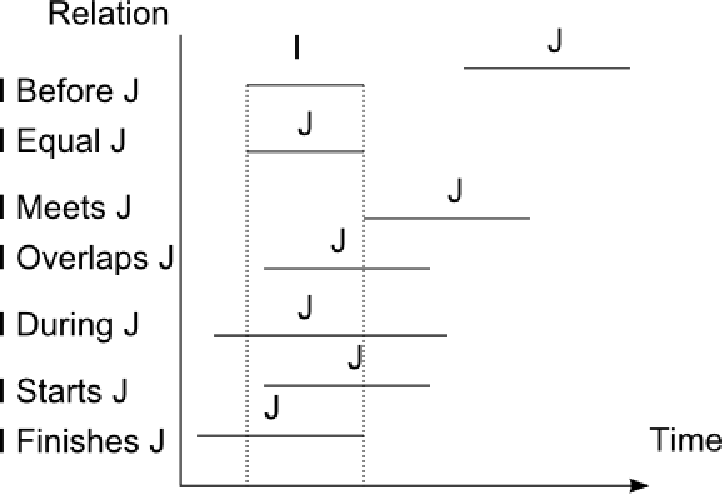
\includegraphics[scale=0.5]{./graphs/allen.pdf}

%}
%\end{center}
%\centerline{ 
\psfig{file=./graphs/Y-time-point.eps}}
%\vspace*{10pt}
%\fcaption{\label{fig:allen-rel}Allen's relations for two crisp time intervals $I$ and $J$.}
%\vspace*{13pt}


%\begin{definition}
%\textbf{Overlaps:}
% \label{def:overlaps}
%Given two time intervals $I = \left(c, d \right)$ and $J = \left(e, f\right)$, it is said that I overlaps J if:
%\begin{equation}
% \label{eqn:overlaps}
%\text{I Overlaps J}  = \left(c > e  \right) \wedge \left(d < f  \right) 
%\end{equation}
%\end{definition}
  

%\begin{definition}
%\textbf{During:}
% \label{def:during}
%Given two time intervals $I = \left(c, d \right)$ and $J = \left(e, f\right)$, it is said that I during J if:
%\begin{equation}
% \label{eqn:during}
%\text{I During J}  = \left(c < e  \right) \wedge \left(d > e  \right) \wedge \left(d < f \right)
%\end{equation}
%\end{definition}

%\begin{definition}
%\textbf{CloseR$\left( I, J \right)$:}
%\label{def:close-a-crisp-interval-r}
%Consider two crisp intervals $I= \left[c ,d \right]$ and $J= \left[e ,f \right]$. The CloseR$\left(I, J\right)$ function allows to close the right-open interval $I$ with respect to the first value $e$ in $J$:
%\begin{align}
%\label{eq:close-a-crisp-interval}
%\mbox{CloseR} \left( I, J \right) &=& \\ 
%\begin{cases}
%\nonumber
%I & \mbox{ if } b \neq +\infty \\
%I=\left[a, c \right[ & \mbox{ if } b = +\infty \wedge J > I
%\left[c, e \right[ & \mbox{ if } d = UC \wedge J \mbox{ During } I \\
%I & \mbox{ in any other case.}
%\end{cases}
%\end{align}
%\end{definition}
